% Options for packages loaded elsewhere
\PassOptionsToPackage{unicode}{hyperref}
\PassOptionsToPackage{hyphens}{url}
%
\documentclass[
]{article}
\title{Lab 08 - Text Mining}
\author{}
\date{\vspace{-2.5em}}

\usepackage{amsmath,amssymb}
\usepackage{lmodern}
\usepackage{iftex}
\ifPDFTeX
  \usepackage[T1]{fontenc}
  \usepackage[utf8]{inputenc}
  \usepackage{textcomp} % provide euro and other symbols
\else % if luatex or xetex
  \usepackage{unicode-math}
  \defaultfontfeatures{Scale=MatchLowercase}
  \defaultfontfeatures[\rmfamily]{Ligatures=TeX,Scale=1}
\fi
% Use upquote if available, for straight quotes in verbatim environments
\IfFileExists{upquote.sty}{\usepackage{upquote}}{}
\IfFileExists{microtype.sty}{% use microtype if available
  \usepackage[]{microtype}
  \UseMicrotypeSet[protrusion]{basicmath} % disable protrusion for tt fonts
}{}
\makeatletter
\@ifundefined{KOMAClassName}{% if non-KOMA class
  \IfFileExists{parskip.sty}{%
    \usepackage{parskip}
  }{% else
    \setlength{\parindent}{0pt}
    \setlength{\parskip}{6pt plus 2pt minus 1pt}}
}{% if KOMA class
  \KOMAoptions{parskip=half}}
\makeatother
\usepackage{xcolor}
\IfFileExists{xurl.sty}{\usepackage{xurl}}{} % add URL line breaks if available
\IfFileExists{bookmark.sty}{\usepackage{bookmark}}{\usepackage{hyperref}}
\hypersetup{
  pdftitle={Lab 08 - Text Mining},
  hidelinks,
  pdfcreator={LaTeX via pandoc}}
\urlstyle{same} % disable monospaced font for URLs
\usepackage[margin=1in]{geometry}
\usepackage{color}
\usepackage{fancyvrb}
\newcommand{\VerbBar}{|}
\newcommand{\VERB}{\Verb[commandchars=\\\{\}]}
\DefineVerbatimEnvironment{Highlighting}{Verbatim}{commandchars=\\\{\}}
% Add ',fontsize=\small' for more characters per line
\usepackage{framed}
\definecolor{shadecolor}{RGB}{248,248,248}
\newenvironment{Shaded}{\begin{snugshade}}{\end{snugshade}}
\newcommand{\AlertTok}[1]{\textcolor[rgb]{0.94,0.16,0.16}{#1}}
\newcommand{\AnnotationTok}[1]{\textcolor[rgb]{0.56,0.35,0.01}{\textbf{\textit{#1}}}}
\newcommand{\AttributeTok}[1]{\textcolor[rgb]{0.77,0.63,0.00}{#1}}
\newcommand{\BaseNTok}[1]{\textcolor[rgb]{0.00,0.00,0.81}{#1}}
\newcommand{\BuiltInTok}[1]{#1}
\newcommand{\CharTok}[1]{\textcolor[rgb]{0.31,0.60,0.02}{#1}}
\newcommand{\CommentTok}[1]{\textcolor[rgb]{0.56,0.35,0.01}{\textit{#1}}}
\newcommand{\CommentVarTok}[1]{\textcolor[rgb]{0.56,0.35,0.01}{\textbf{\textit{#1}}}}
\newcommand{\ConstantTok}[1]{\textcolor[rgb]{0.00,0.00,0.00}{#1}}
\newcommand{\ControlFlowTok}[1]{\textcolor[rgb]{0.13,0.29,0.53}{\textbf{#1}}}
\newcommand{\DataTypeTok}[1]{\textcolor[rgb]{0.13,0.29,0.53}{#1}}
\newcommand{\DecValTok}[1]{\textcolor[rgb]{0.00,0.00,0.81}{#1}}
\newcommand{\DocumentationTok}[1]{\textcolor[rgb]{0.56,0.35,0.01}{\textbf{\textit{#1}}}}
\newcommand{\ErrorTok}[1]{\textcolor[rgb]{0.64,0.00,0.00}{\textbf{#1}}}
\newcommand{\ExtensionTok}[1]{#1}
\newcommand{\FloatTok}[1]{\textcolor[rgb]{0.00,0.00,0.81}{#1}}
\newcommand{\FunctionTok}[1]{\textcolor[rgb]{0.00,0.00,0.00}{#1}}
\newcommand{\ImportTok}[1]{#1}
\newcommand{\InformationTok}[1]{\textcolor[rgb]{0.56,0.35,0.01}{\textbf{\textit{#1}}}}
\newcommand{\KeywordTok}[1]{\textcolor[rgb]{0.13,0.29,0.53}{\textbf{#1}}}
\newcommand{\NormalTok}[1]{#1}
\newcommand{\OperatorTok}[1]{\textcolor[rgb]{0.81,0.36,0.00}{\textbf{#1}}}
\newcommand{\OtherTok}[1]{\textcolor[rgb]{0.56,0.35,0.01}{#1}}
\newcommand{\PreprocessorTok}[1]{\textcolor[rgb]{0.56,0.35,0.01}{\textit{#1}}}
\newcommand{\RegionMarkerTok}[1]{#1}
\newcommand{\SpecialCharTok}[1]{\textcolor[rgb]{0.00,0.00,0.00}{#1}}
\newcommand{\SpecialStringTok}[1]{\textcolor[rgb]{0.31,0.60,0.02}{#1}}
\newcommand{\StringTok}[1]{\textcolor[rgb]{0.31,0.60,0.02}{#1}}
\newcommand{\VariableTok}[1]{\textcolor[rgb]{0.00,0.00,0.00}{#1}}
\newcommand{\VerbatimStringTok}[1]{\textcolor[rgb]{0.31,0.60,0.02}{#1}}
\newcommand{\WarningTok}[1]{\textcolor[rgb]{0.56,0.35,0.01}{\textbf{\textit{#1}}}}
\usepackage{graphicx}
\makeatletter
\def\maxwidth{\ifdim\Gin@nat@width>\linewidth\linewidth\else\Gin@nat@width\fi}
\def\maxheight{\ifdim\Gin@nat@height>\textheight\textheight\else\Gin@nat@height\fi}
\makeatother
% Scale images if necessary, so that they will not overflow the page
% margins by default, and it is still possible to overwrite the defaults
% using explicit options in \includegraphics[width, height, ...]{}
\setkeys{Gin}{width=\maxwidth,height=\maxheight,keepaspectratio}
% Set default figure placement to htbp
\makeatletter
\def\fps@figure{htbp}
\makeatother
\setlength{\emergencystretch}{3em} % prevent overfull lines
\providecommand{\tightlist}{%
  \setlength{\itemsep}{0pt}\setlength{\parskip}{0pt}}
\setcounter{secnumdepth}{-\maxdimen} % remove section numbering
\usepackage{booktabs}
\usepackage{longtable}
\usepackage{array}
\usepackage{multirow}
\usepackage{wrapfig}
\usepackage{float}
\usepackage{colortbl}
\usepackage{pdflscape}
\usepackage{tabu}
\usepackage{threeparttable}
\usepackage{threeparttablex}
\usepackage[normalem]{ulem}
\usepackage{makecell}
\usepackage{xcolor}
\ifLuaTeX
  \usepackage{selnolig}  % disable illegal ligatures
\fi

\begin{document}
\maketitle

\begin{Shaded}
\begin{Highlighting}[]
\NormalTok{knitr}\SpecialCharTok{::}\NormalTok{opts\_chunk}\SpecialCharTok{$}\FunctionTok{set}\NormalTok{(}\AttributeTok{eval =}\NormalTok{ T, }\AttributeTok{include  =}\NormalTok{ T)}
\end{Highlighting}
\end{Shaded}

\hypertarget{learning-goals}{%
\section{Learning goals}\label{learning-goals}}

\begin{itemize}
\tightlist
\item
  Use \texttt{unnest\_tokens()} and \texttt{unnest\_ngrams()} to extract
  tokens and ngrams from text.
\item
  Use dplyr and ggplot2 to analyze text data
\end{itemize}

\hypertarget{lab-description}{%
\section{Lab description}\label{lab-description}}

For this lab we will be working with the medical record transcriptions
from \url{https://www.mtsamples.com/}. And is loaded and ``fairly''
cleaned at
\url{https://github.com/JSC370/jsc370-2022/blob/main/data/medical_transcriptions/mtsamples.csv}.

This markdown document should be rendered using
\texttt{github\_document} document.

\hypertarget{setup-packages}{%
\subsubsection{Setup packages}\label{setup-packages}}

You should load in \texttt{dplyr}, (or \texttt{data.table} if you want
to work that way), \texttt{ggplot2} and \texttt{tidytext}. If you don't
already have \texttt{tidytext} then you can install with

\begin{Shaded}
\begin{Highlighting}[]
\FunctionTok{install.packages}\NormalTok{(}\StringTok{"tidytext"}\NormalTok{)}
\end{Highlighting}
\end{Shaded}

\hypertarget{read-in-medical-transcriptions}{%
\subsubsection{read in Medical
Transcriptions}\label{read-in-medical-transcriptions}}

Loading in reference transcription samples from
\url{https://www.mtsamples.com/}

\begin{Shaded}
\begin{Highlighting}[]
\FunctionTok{library}\NormalTok{(tidytext)}
\FunctionTok{library}\NormalTok{(readr)}
\FunctionTok{library}\NormalTok{(dplyr)}
\FunctionTok{library}\NormalTok{(tidyr)}
\FunctionTok{library}\NormalTok{(ggplot2)}
\FunctionTok{library}\NormalTok{(wordcloud)}
\FunctionTok{library}\NormalTok{(kableExtra)}

\NormalTok{mt\_samples }\OtherTok{\textless{}{-}} \FunctionTok{read\_csv}\NormalTok{(}\StringTok{"https://raw.githubusercontent.com/JSC370/jsc370{-}2022/main/data/medical\_transcriptions/mtsamples.csv"}\NormalTok{)}
\NormalTok{mt\_samples }\OtherTok{\textless{}{-}}\NormalTok{ mt\_samples }\SpecialCharTok{\%\textgreater{}\%}
  \FunctionTok{select}\NormalTok{(description, medical\_specialty, transcription)}

\FunctionTok{head}\NormalTok{(mt\_samples)}
\end{Highlighting}
\end{Shaded}

\begin{verbatim}
## # A tibble: 6 x 3
##   description                  medical_specialty   transcription                
##   <chr>                        <chr>               <chr>                        
## 1 A 23-year-old white female ~ Allergy / Immunolo~ "SUBJECTIVE:,  This 23-year-~
## 2 Consult for laparoscopic ga~ Bariatrics          "PAST MEDICAL HISTORY:, He h~
## 3 Consult for laparoscopic ga~ Bariatrics          "HISTORY OF PRESENT ILLNESS:~
## 4 2-D M-Mode. Doppler.         Cardiovascular / P~ "2-D M-MODE: , ,1.  Left atr~
## 5 2-D Echocardiogram           Cardiovascular / P~ "1.  The left ventricular ca~
## 6 Morbid obesity.  Laparoscop~ Bariatrics          "PREOPERATIVE DIAGNOSIS: , M~
\end{verbatim}

\begin{center}\rule{0.5\linewidth}{0.5pt}\end{center}

\hypertarget{question-1-what-specialties-do-we-have}{%
\subsection{Question 1: What specialties do we
have?}\label{question-1-what-specialties-do-we-have}}

We can use \texttt{count()} from \texttt{dplyr} to figure out how many
different catagories do we have? Are these catagories related?
overlapping? evenly distributed?

\begin{Shaded}
\begin{Highlighting}[]
\NormalTok{mt\_samples }\SpecialCharTok{\%\textgreater{}\%}
  \FunctionTok{count}\NormalTok{(medical\_specialty, }\AttributeTok{sort =} \ConstantTok{TRUE}\NormalTok{) }\SpecialCharTok{\%\textgreater{}\%}
  \FunctionTok{ggplot}\NormalTok{(}\FunctionTok{aes}\NormalTok{(medical\_specialty, n)) }\SpecialCharTok{+}
  \FunctionTok{geom\_col}\NormalTok{() }\SpecialCharTok{+} 
  \FunctionTok{coord\_flip}\NormalTok{()}
\end{Highlighting}
\end{Shaded}

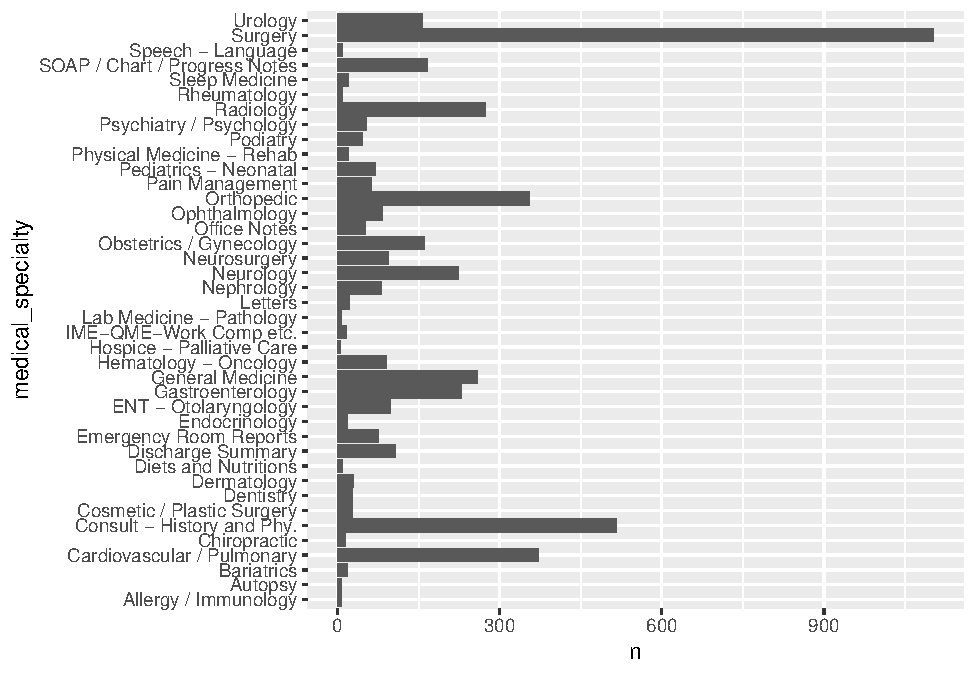
\includegraphics{lab08-text-mining_files/figure-latex/unnamed-chunk-3-1.pdf}

By looking at the above barplot, we can see there are 40 total
categories in the dataset, and while some (such as surgery) are more
frequent than others, there seems to be a somewhat even distribution of
categories.

\begin{center}\rule{0.5\linewidth}{0.5pt}\end{center}

\hypertarget{question-2}{%
\subsection{Question 2}\label{question-2}}

\begin{itemize}
\tightlist
\item
  Tokenize the the words in the \texttt{transcription} column
\item
  Count the number of times each token appears
\item
  Visualize the top 20 most frequent words
\end{itemize}

\begin{Shaded}
\begin{Highlighting}[]
\NormalTok{tokens }\OtherTok{\textless{}{-}}\NormalTok{ mt\_samples }\SpecialCharTok{\%\textgreater{}\%}
  \FunctionTok{select}\NormalTok{(transcription) }\SpecialCharTok{\%\textgreater{}\%}
  \FunctionTok{unnest\_tokens}\NormalTok{(word, transcription) }\SpecialCharTok{\%\textgreater{}\%}
  \FunctionTok{group\_by}\NormalTok{(word) }\SpecialCharTok{\%\textgreater{}\%}
  \FunctionTok{summarise}\NormalTok{(}\AttributeTok{word\_frequency =} \FunctionTok{n}\NormalTok{()) }\SpecialCharTok{\%\textgreater{}\%}
  \FunctionTok{arrange}\NormalTok{(}\FunctionTok{across}\NormalTok{(word\_frequency, desc)) }\SpecialCharTok{\%\textgreater{}\%}
  \FunctionTok{head}\NormalTok{(}\DecValTok{20}\NormalTok{)}

\NormalTok{tokens }\SpecialCharTok{\%\textgreater{}\%}
  \FunctionTok{kable}\NormalTok{() }\SpecialCharTok{\%\textgreater{}\%}
  \FunctionTok{kable\_styling}\NormalTok{()}
\end{Highlighting}
\end{Shaded}

\begin{table}
\centering
\begin{tabular}{l|r}
\hline
word & word\_frequency\\
\hline
the & 149888\\
\hline
and & 82779\\
\hline
was & 71765\\
\hline
of & 59205\\
\hline
to & 50632\\
\hline
a & 42810\\
\hline
with & 35815\\
\hline
in & 32807\\
\hline
is & 26378\\
\hline
patient & 22065\\
\hline
no & 17874\\
\hline
she & 17593\\
\hline
for & 17049\\
\hline
he & 15542\\
\hline
were & 15535\\
\hline
on & 14694\\
\hline
this & 13949\\
\hline
at & 13492\\
\hline
then & 12430\\
\hline
right & 11587\\
\hline
\end{tabular}
\end{table}

Above, we can see the top 20 words and their associated frequencies.
Next, we will draw a barplot describing these frequencies:

\begin{Shaded}
\begin{Highlighting}[]
\NormalTok{tokens }\SpecialCharTok{\%\textgreater{}\%}
  \FunctionTok{ggplot}\NormalTok{(}\FunctionTok{aes}\NormalTok{(}\FunctionTok{reorder}\NormalTok{(word, }\SpecialCharTok{{-}}\NormalTok{word\_frequency), word\_frequency)) }\SpecialCharTok{+}
  \FunctionTok{geom\_bar}\NormalTok{(}\AttributeTok{stat =} \StringTok{\textquotesingle{}identity\textquotesingle{}}\NormalTok{)}
\end{Highlighting}
\end{Shaded}

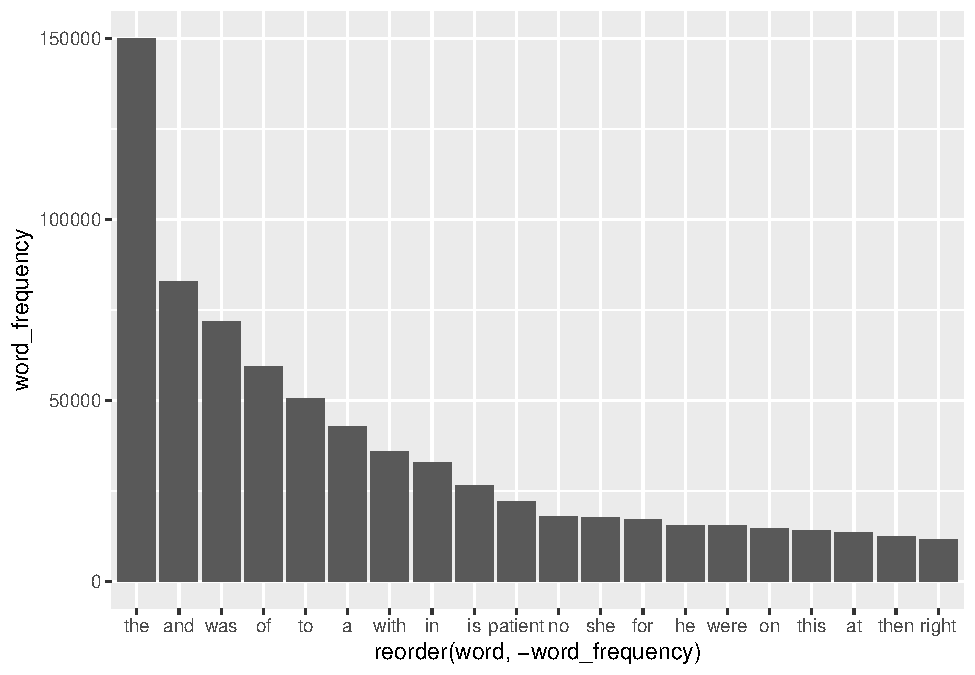
\includegraphics{lab08-text-mining_files/figure-latex/unnamed-chunk-5-1.pdf}

We can also draw a (currently not so interesting) Wordcloud
visualization of these words:

\begin{Shaded}
\begin{Highlighting}[]
\FunctionTok{wordcloud}\NormalTok{(tokens}\SpecialCharTok{$}\NormalTok{word, tokens}\SpecialCharTok{$}\NormalTok{word\_frequency)}
\end{Highlighting}
\end{Shaded}

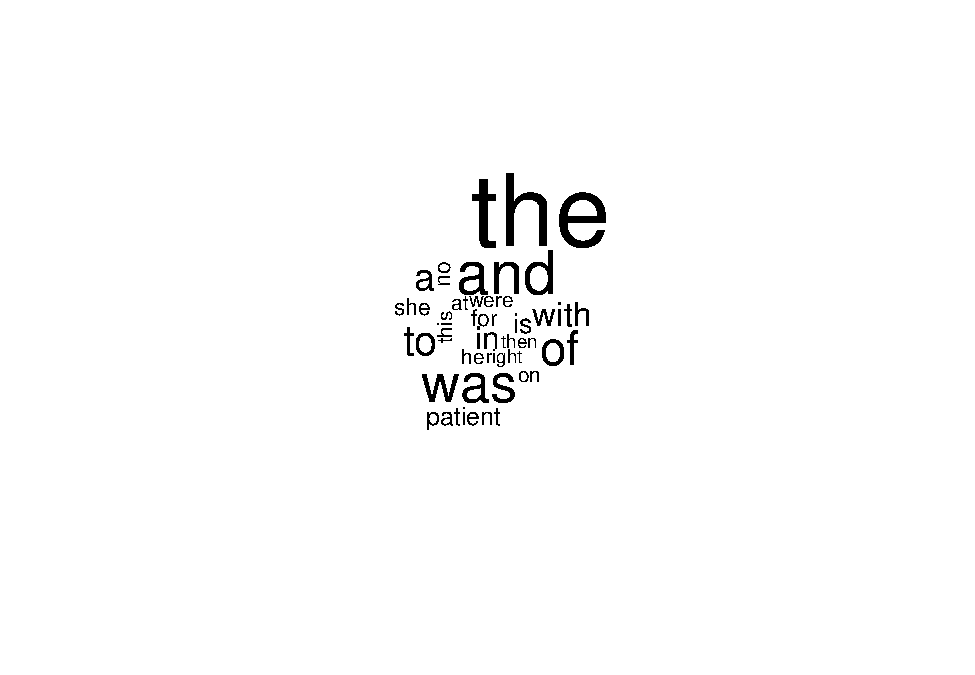
\includegraphics{lab08-text-mining_files/figure-latex/unnamed-chunk-6-1.pdf}

Explain what we see from this result. Does it makes sense? What insights
(if any) do we get?

The results we get from tokenizing make sense as words such as the, and,
was, and so on are typically assumed to be frequently occurring in
English medical journals. However, we don't gain much insight from this
as knowing these regular English words are the most prevalent doesn't
tell us much about the contents of these journals, the categories to
which they belong, or frankly any other useful information.

\begin{center}\rule{0.5\linewidth}{0.5pt}\end{center}

\hypertarget{question-3}{%
\subsection{Question 3}\label{question-3}}

\begin{itemize}
\tightlist
\item
  Redo visualization but remove stopwords before
\item
  Bonus points if you remove numbers as well
\end{itemize}

\begin{Shaded}
\begin{Highlighting}[]
\NormalTok{tokens }\OtherTok{\textless{}{-}}\NormalTok{ mt\_samples }\SpecialCharTok{\%\textgreater{}\%}
  \FunctionTok{select}\NormalTok{(transcription) }\SpecialCharTok{\%\textgreater{}\%}
  \FunctionTok{unnest\_tokens}\NormalTok{(word, transcription) }\SpecialCharTok{\%\textgreater{}\%}
  \FunctionTok{anti\_join}\NormalTok{(stop\_words, }\AttributeTok{by=}\StringTok{"word"}\NormalTok{) }\SpecialCharTok{\%\textgreater{}\%}
  \FunctionTok{subset}\NormalTok{(}\SpecialCharTok{!}\FunctionTok{grepl}\NormalTok{(}\StringTok{"\^{}}\SpecialCharTok{\textbackslash{}\textbackslash{}}\StringTok{d+$"}\NormalTok{, word)) }\SpecialCharTok{\%\textgreater{}\%}
  \FunctionTok{group\_by}\NormalTok{(word) }\SpecialCharTok{\%\textgreater{}\%}
  \FunctionTok{summarise}\NormalTok{(}\AttributeTok{word\_frequency =} \FunctionTok{n}\NormalTok{()) }\SpecialCharTok{\%\textgreater{}\%}
  \FunctionTok{arrange}\NormalTok{(}\FunctionTok{across}\NormalTok{(word\_frequency, desc)) }\SpecialCharTok{\%\textgreater{}\%}
  \FunctionTok{head}\NormalTok{(}\DecValTok{20}\NormalTok{)}

\NormalTok{tokens }\SpecialCharTok{\%\textgreater{}\%}
  \FunctionTok{kable}\NormalTok{() }\SpecialCharTok{\%\textgreater{}\%}
  \FunctionTok{kable\_styling}\NormalTok{()}
\end{Highlighting}
\end{Shaded}

\begin{table}
\centering
\begin{tabular}{l|r}
\hline
word & word\_frequency\\
\hline
patient & 22065\\
\hline
left & 11258\\
\hline
history & 9509\\
\hline
normal & 7526\\
\hline
procedure & 7463\\
\hline
pain & 5976\\
\hline
noted & 4348\\
\hline
time & 4287\\
\hline
mg & 4087\\
\hline
blood & 3956\\
\hline
performed & 3953\\
\hline
skin & 3798\\
\hline
anesthesia & 3707\\
\hline
incision & 3601\\
\hline
removed & 3532\\
\hline
diagnosis & 3212\\
\hline
artery & 3027\\
\hline
anterior & 2932\\
\hline
disease & 2682\\
\hline
past & 2674\\
\hline
\end{tabular}
\end{table}

Above, we can see the top 20 words and their associated frequencies
AFTER filtering out stopwords. Next, we will draw a barplot describing
these frequencies:

\begin{Shaded}
\begin{Highlighting}[]
\NormalTok{tokens }\SpecialCharTok{\%\textgreater{}\%}
  \FunctionTok{ggplot}\NormalTok{(}\FunctionTok{aes}\NormalTok{(}\FunctionTok{reorder}\NormalTok{(word, }\SpecialCharTok{{-}}\NormalTok{word\_frequency), word\_frequency)) }\SpecialCharTok{+}
  \FunctionTok{geom\_bar}\NormalTok{(}\AttributeTok{stat =} \StringTok{\textquotesingle{}identity\textquotesingle{}}\NormalTok{) }\SpecialCharTok{+}
  \FunctionTok{coord\_flip}\NormalTok{()}
\end{Highlighting}
\end{Shaded}

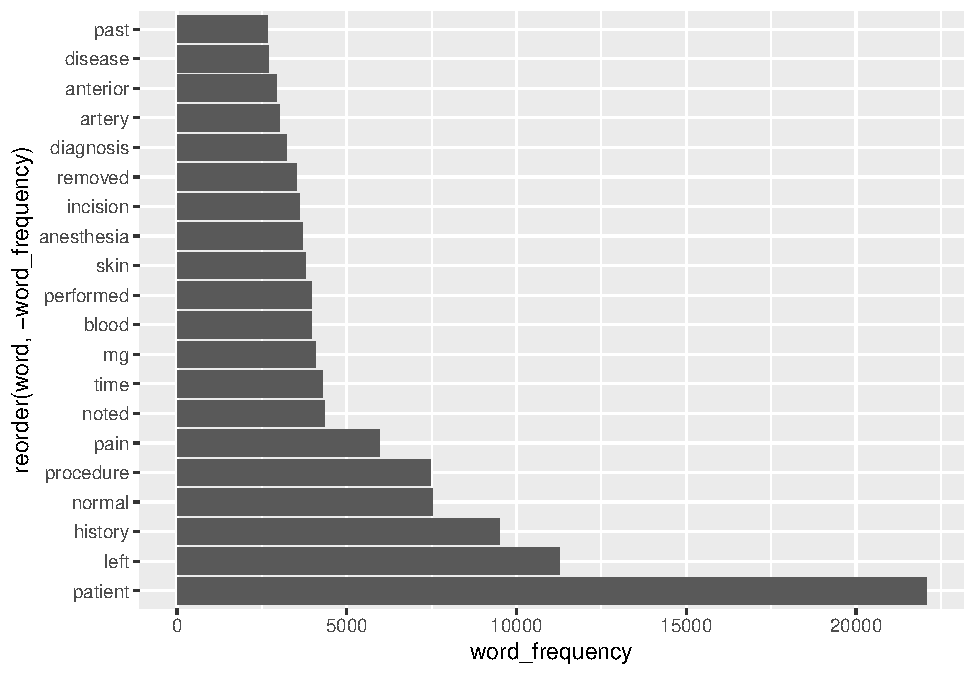
\includegraphics{lab08-text-mining_files/figure-latex/unnamed-chunk-8-1.pdf}

We can also draw a (now a little more interesting) Wordcloud
visualization of these words:

\begin{Shaded}
\begin{Highlighting}[]
\FunctionTok{wordcloud}\NormalTok{(tokens}\SpecialCharTok{$}\NormalTok{word, tokens}\SpecialCharTok{$}\NormalTok{word\_frequency)}
\end{Highlighting}
\end{Shaded}

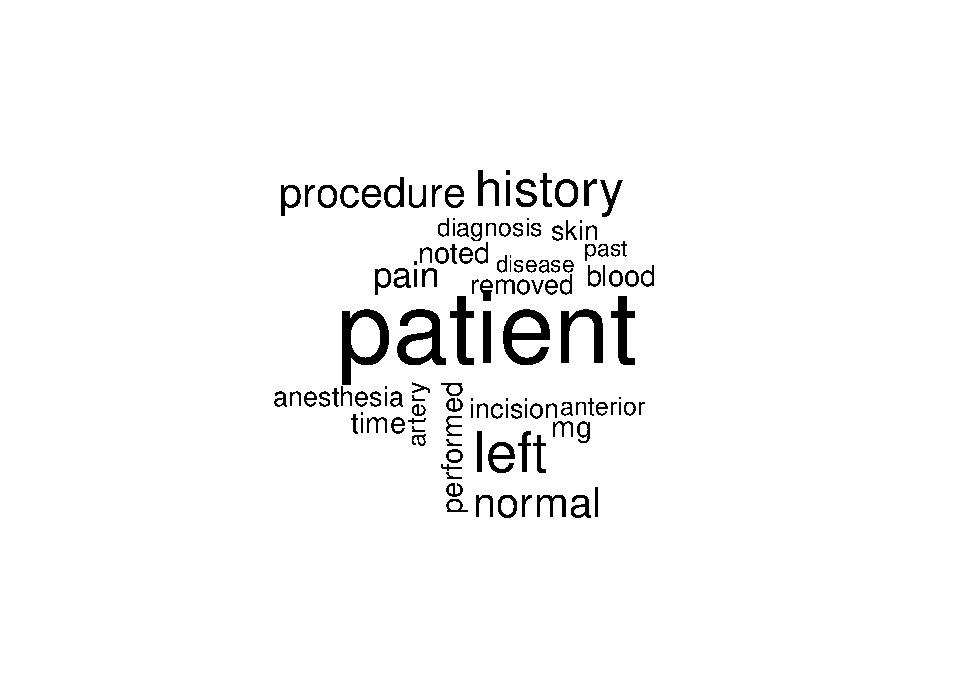
\includegraphics{lab08-text-mining_files/figure-latex/unnamed-chunk-9-1.pdf}

What do we see know that we have removed stop words? Does it give us a
better idea of what the text is about?

By removing stopwords we can indeed start to see some more interesting
results about what words appear the most frequently. That is, it is now
a lot clearer that we are looking through medical journals with words
such as ``patient'', ``procedure'', and ``diagnosis'' appearing very
frequently.

\begin{center}\rule{0.5\linewidth}{0.5pt}\end{center}

\hypertarget{question-4}{%
\section{Question 4}\label{question-4}}

Repeat question 2, but this time tokenize into bi-grams. How does the
result change if you look at tri-grams?

We will first consider bigrams:

\begin{Shaded}
\begin{Highlighting}[]
\NormalTok{tokens }\OtherTok{\textless{}{-}}\NormalTok{ mt\_samples }\SpecialCharTok{\%\textgreater{}\%}
  \FunctionTok{select}\NormalTok{(transcription) }\SpecialCharTok{\%\textgreater{}\%}
  \FunctionTok{unnest\_tokens}\NormalTok{(bigram, transcription, }\AttributeTok{token =} \StringTok{"ngrams"}\NormalTok{, }\AttributeTok{n =} \DecValTok{2}\NormalTok{) }\SpecialCharTok{\%\textgreater{}\%}
  \FunctionTok{group\_by}\NormalTok{(bigram) }\SpecialCharTok{\%\textgreater{}\%}
  \FunctionTok{summarise}\NormalTok{(}\AttributeTok{bigram\_frequency =} \FunctionTok{n}\NormalTok{()) }\SpecialCharTok{\%\textgreater{}\%}
  \FunctionTok{separate}\NormalTok{(bigram, }
           \FunctionTok{c}\NormalTok{(}\StringTok{"word1"}\NormalTok{, }\StringTok{"word2"}\NormalTok{), }
           \AttributeTok{extra =} \StringTok{"drop"}\NormalTok{, }
           \AttributeTok{remove =} \ConstantTok{FALSE}\NormalTok{, }
           \AttributeTok{sep =} \StringTok{" "}\NormalTok{, }
           \AttributeTok{fill =} \StringTok{"right"}\NormalTok{) }\SpecialCharTok{\%\textgreater{}\%}
  \FunctionTok{anti\_join}\NormalTok{(stop\_words, }\AttributeTok{by =} \FunctionTok{c}\NormalTok{(}\StringTok{"word1"} \OtherTok{=} \StringTok{"word"}\NormalTok{)) }\SpecialCharTok{\%\textgreater{}\%}
  \FunctionTok{anti\_join}\NormalTok{(stop\_words, }\AttributeTok{by =} \FunctionTok{c}\NormalTok{(}\StringTok{"word2"} \OtherTok{=} \StringTok{"word"}\NormalTok{)) }\SpecialCharTok{\%\textgreater{}\%}
  \FunctionTok{subset}\NormalTok{(}\SpecialCharTok{!}\FunctionTok{grepl}\NormalTok{(}\StringTok{"}\SpecialCharTok{\textbackslash{}\textbackslash{}}\StringTok{d+"}\NormalTok{, bigram)) }\SpecialCharTok{\%\textgreater{}\%}
  \FunctionTok{arrange}\NormalTok{(}\FunctionTok{across}\NormalTok{(bigram\_frequency, desc)) }\SpecialCharTok{\%\textgreater{}\%}
  \FunctionTok{head}\NormalTok{(}\DecValTok{20}\NormalTok{)}

\NormalTok{tokens }\SpecialCharTok{\%\textgreater{}\%}
  \FunctionTok{kable}\NormalTok{() }\SpecialCharTok{\%\textgreater{}\%}
  \FunctionTok{kable\_styling}\NormalTok{()}
\end{Highlighting}
\end{Shaded}

\begin{table}
\centering
\begin{tabular}{l|l|l|r}
\hline
bigram & word1 & word2 & bigram\_frequency\\
\hline
blood pressure & blood & pressure & 1265\\
\hline
medical history & medical & history & 1223\\
\hline
preoperative diagnosis & preoperative & diagnosis & 1176\\
\hline
physical examination & physical & examination & 1156\\
\hline
vital signs & vital & signs & 1121\\
\hline
past medical & past & medical & 1113\\
\hline
postoperative diagnosis & postoperative & diagnosis & 1092\\
\hline
coronary artery & coronary & artery & 1032\\
\hline
patient tolerated & patient & tolerated & 994\\
\hline
blood loss & blood & loss & 965\\
\hline
family history & family & history & 941\\
\hline
social history & social & history & 865\\
\hline
stable condition & stable & condition & 835\\
\hline
supine position & supine & position & 786\\
\hline
status post & status & post & 783\\
\hline
estimated blood & estimated & blood & 754\\
\hline
sterile fashion & sterile & fashion & 721\\
\hline
mg p.o & mg & p.o & 718\\
\hline
chest pain & chest & pain & 707\\
\hline
informed consent & informed & consent & 685\\
\hline
\end{tabular}
\end{table}

Above, we can see the top 20 bigrams and their associated frequencies
AFTER filtering out stopwords. Next, we will draw a barplot describing
these frequencies:

\begin{Shaded}
\begin{Highlighting}[]
\NormalTok{tokens }\SpecialCharTok{\%\textgreater{}\%}
  \FunctionTok{ggplot}\NormalTok{(}\FunctionTok{aes}\NormalTok{(}\FunctionTok{reorder}\NormalTok{(bigram, }\SpecialCharTok{{-}}\NormalTok{bigram\_frequency), bigram\_frequency)) }\SpecialCharTok{+}
  \FunctionTok{geom\_bar}\NormalTok{(}\AttributeTok{stat =} \StringTok{\textquotesingle{}identity\textquotesingle{}}\NormalTok{) }\SpecialCharTok{+}
  \FunctionTok{coord\_flip}\NormalTok{()}
\end{Highlighting}
\end{Shaded}

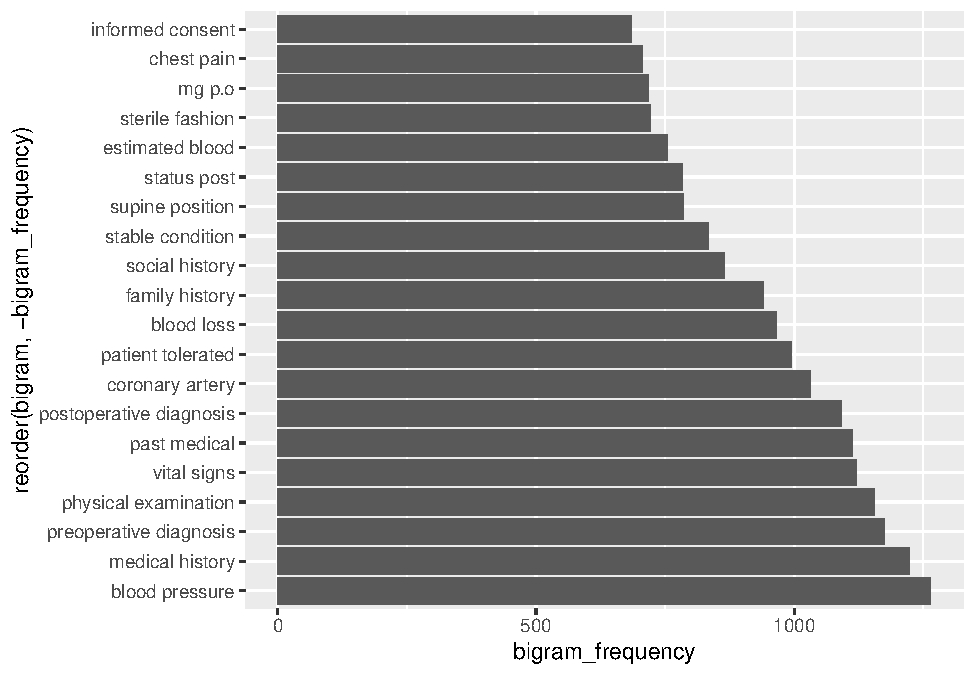
\includegraphics{lab08-text-mining_files/figure-latex/unnamed-chunk-11-1.pdf}

Now, we will do the exact same thing but with trigrams:

\begin{Shaded}
\begin{Highlighting}[]
\NormalTok{tokens }\OtherTok{\textless{}{-}}\NormalTok{ mt\_samples }\SpecialCharTok{\%\textgreater{}\%}
  \FunctionTok{select}\NormalTok{(transcription) }\SpecialCharTok{\%\textgreater{}\%}
  \FunctionTok{unnest\_tokens}\NormalTok{(trigram, transcription, }\AttributeTok{token =} \StringTok{"ngrams"}\NormalTok{, }\AttributeTok{n =} \DecValTok{3}\NormalTok{) }\SpecialCharTok{\%\textgreater{}\%}
  \FunctionTok{group\_by}\NormalTok{(trigram) }\SpecialCharTok{\%\textgreater{}\%}
  \FunctionTok{summarise}\NormalTok{(}\AttributeTok{trigram\_frequency =} \FunctionTok{n}\NormalTok{()) }\SpecialCharTok{\%\textgreater{}\%}
  \FunctionTok{separate}\NormalTok{(trigram, }
           \FunctionTok{c}\NormalTok{(}\StringTok{"word1"}\NormalTok{, }\StringTok{"word2"}\NormalTok{, }\StringTok{"word3"}\NormalTok{), }
           \AttributeTok{extra =} \StringTok{"drop"}\NormalTok{, }
           \AttributeTok{remove =} \ConstantTok{FALSE}\NormalTok{, }
           \AttributeTok{sep =} \StringTok{" "}\NormalTok{, }
           \AttributeTok{fill =} \StringTok{"right"}\NormalTok{) }\SpecialCharTok{\%\textgreater{}\%}
  \FunctionTok{anti\_join}\NormalTok{(stop\_words, }\AttributeTok{by =} \FunctionTok{c}\NormalTok{(}\StringTok{"word1"} \OtherTok{=} \StringTok{"word"}\NormalTok{)) }\SpecialCharTok{\%\textgreater{}\%}
  \FunctionTok{anti\_join}\NormalTok{(stop\_words, }\AttributeTok{by =} \FunctionTok{c}\NormalTok{(}\StringTok{"word2"} \OtherTok{=} \StringTok{"word"}\NormalTok{)) }\SpecialCharTok{\%\textgreater{}\%}
  \FunctionTok{anti\_join}\NormalTok{(stop\_words, }\AttributeTok{by =} \FunctionTok{c}\NormalTok{(}\StringTok{"word3"} \OtherTok{=} \StringTok{"word"}\NormalTok{)) }\SpecialCharTok{\%\textgreater{}\%}
  \FunctionTok{subset}\NormalTok{(}\SpecialCharTok{!}\FunctionTok{grepl}\NormalTok{(}\StringTok{"}\SpecialCharTok{\textbackslash{}\textbackslash{}}\StringTok{d+"}\NormalTok{, trigram)) }\SpecialCharTok{\%\textgreater{}\%}
  \FunctionTok{arrange}\NormalTok{(}\FunctionTok{across}\NormalTok{(trigram\_frequency, desc)) }\SpecialCharTok{\%\textgreater{}\%}
  \FunctionTok{head}\NormalTok{(}\DecValTok{20}\NormalTok{)}

\NormalTok{tokens }\SpecialCharTok{\%\textgreater{}\%}
  \FunctionTok{kable}\NormalTok{() }\SpecialCharTok{\%\textgreater{}\%}
  \FunctionTok{kable\_styling}\NormalTok{()}
\end{Highlighting}
\end{Shaded}

\begin{table}
\centering
\begin{tabular}{l|l|l|l|r}
\hline
trigram & word1 & word2 & word3 & trigram\_frequency\\
\hline
past medical history & past & medical & history & 1063\\
\hline
estimated blood loss & estimated & blood & loss & 754\\
\hline
coronary artery disease & coronary & artery & disease & 419\\
\hline
past surgical history & past & surgical & history & 419\\
\hline
examination vital signs & examination & vital & signs & 404\\
\hline
physical examination vital & physical & examination & vital & 404\\
\hline
usual sterile fashion & usual & sterile & fashion & 376\\
\hline
mg p.o daily & mg & p.o & daily & 273\\
\hline
left anterior descending & left & anterior & descending & 269\\
\hline
left lower extremity & left & lower & extremity & 192\\
\hline
heart regular rate & heart & regular & rate & 189\\
\hline
blood loss minimal & blood & loss & minimal & 176\\
\hline
abdomen soft nontender & abdomen & soft & nontender & 172\\
\hline
vital signs blood & vital & signs & blood & 170\\
\hline
congestive heart failure & congestive & heart & failure & 169\\
\hline
signs blood pressure & signs & blood & pressure & 167\\
\hline
normal sinus rhythm & normal & sinus & rhythm & 162\\
\hline
cranial nerves ii & cranial & nerves & ii & 159\\
\hline
transverse carpal ligament & transverse & carpal & ligament & 159\\
\hline
vital signs temperature & vital & signs & temperature & 156\\
\hline
\end{tabular}
\end{table}

Above, we can see the top 20 trigrams and their associated frequencies
AFTER filtering out stopwords. Next, we will draw a barplot describing
these frequencies:

\begin{Shaded}
\begin{Highlighting}[]
\NormalTok{tokens }\SpecialCharTok{\%\textgreater{}\%}
  \FunctionTok{ggplot}\NormalTok{(}\FunctionTok{aes}\NormalTok{(}\FunctionTok{reorder}\NormalTok{(trigram, }\SpecialCharTok{{-}}\NormalTok{trigram\_frequency), trigram\_frequency)) }\SpecialCharTok{+}
  \FunctionTok{geom\_bar}\NormalTok{(}\AttributeTok{stat =} \StringTok{\textquotesingle{}identity\textquotesingle{}}\NormalTok{) }\SpecialCharTok{+}
  \FunctionTok{coord\_flip}\NormalTok{()}
\end{Highlighting}
\end{Shaded}

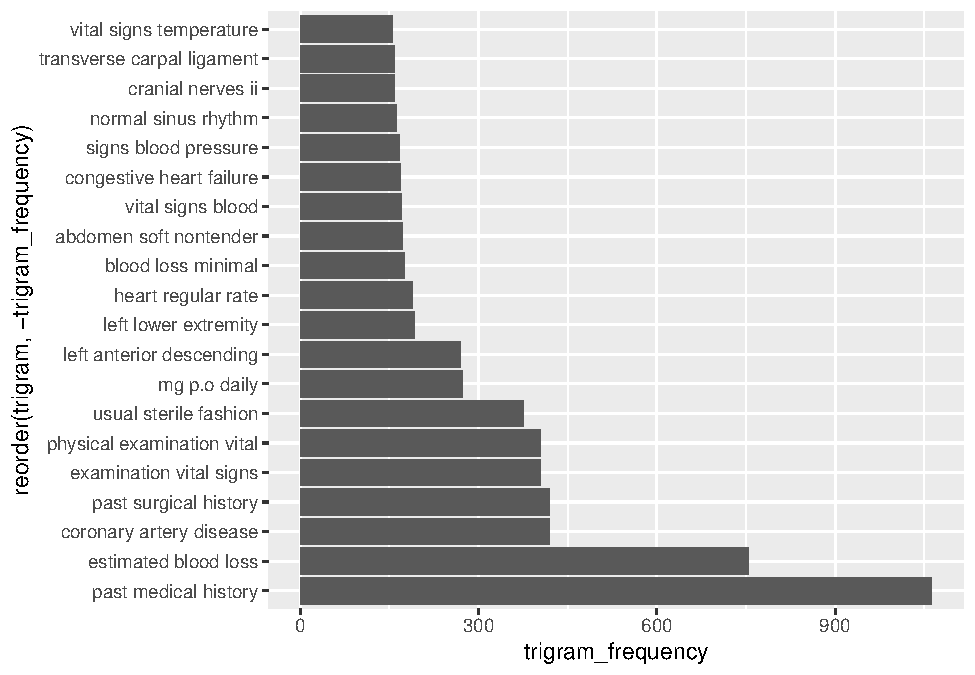
\includegraphics{lab08-text-mining_files/figure-latex/unnamed-chunk-13-1.pdf}

We can see that the results change somewhat after transitioning from
bigrams to trigrams, which makes sense because chunks of 3 words will
probably have different frequencies than chunks of 2 words. This could
be for many reasons, such as some of the more frequent bigrams having a
stop word immediately following (i.e.~``blood loss of''), which would
make the corresponding trigram ineligible to be included in our count.

\begin{center}\rule{0.5\linewidth}{0.5pt}\end{center}

\hypertarget{question-5}{%
\section{Question 5}\label{question-5}}

Using the results you got from question 4. Pick a word and count the
words that appears after and before it.

First, reset \texttt{tokens} to hold all the trigrams and not just the
top 20:

\begin{Shaded}
\begin{Highlighting}[]
\NormalTok{tokens }\OtherTok{\textless{}{-}}\NormalTok{ mt\_samples }\SpecialCharTok{\%\textgreater{}\%}
  \FunctionTok{select}\NormalTok{(transcription) }\SpecialCharTok{\%\textgreater{}\%}
  \FunctionTok{unnest\_tokens}\NormalTok{(trigram, transcription, }\AttributeTok{token =} \StringTok{"ngrams"}\NormalTok{, }\AttributeTok{n =} \DecValTok{3}\NormalTok{) }\SpecialCharTok{\%\textgreater{}\%}
  \FunctionTok{group\_by}\NormalTok{(trigram) }\SpecialCharTok{\%\textgreater{}\%}
  \FunctionTok{summarise}\NormalTok{(}\AttributeTok{trigram\_frequency =} \FunctionTok{n}\NormalTok{()) }\SpecialCharTok{\%\textgreater{}\%}
  \FunctionTok{separate}\NormalTok{(trigram, }
           \FunctionTok{c}\NormalTok{(}\StringTok{"word1"}\NormalTok{, }\StringTok{"word2"}\NormalTok{, }\StringTok{"word3"}\NormalTok{), }
           \AttributeTok{extra =} \StringTok{"drop"}\NormalTok{, }
           \AttributeTok{remove =} \ConstantTok{FALSE}\NormalTok{, }
           \AttributeTok{sep =} \StringTok{" "}\NormalTok{, }
           \AttributeTok{fill =} \StringTok{"right"}\NormalTok{) }\SpecialCharTok{\%\textgreater{}\%}
  \FunctionTok{anti\_join}\NormalTok{(stop\_words, }\AttributeTok{by =} \FunctionTok{c}\NormalTok{(}\StringTok{"word1"} \OtherTok{=} \StringTok{"word"}\NormalTok{)) }\SpecialCharTok{\%\textgreater{}\%}
  \FunctionTok{anti\_join}\NormalTok{(stop\_words, }\AttributeTok{by =} \FunctionTok{c}\NormalTok{(}\StringTok{"word2"} \OtherTok{=} \StringTok{"word"}\NormalTok{)) }\SpecialCharTok{\%\textgreater{}\%}
  \FunctionTok{anti\_join}\NormalTok{(stop\_words, }\AttributeTok{by =} \FunctionTok{c}\NormalTok{(}\StringTok{"word3"} \OtherTok{=} \StringTok{"word"}\NormalTok{)) }\SpecialCharTok{\%\textgreater{}\%}
  \FunctionTok{subset}\NormalTok{(}\SpecialCharTok{!}\FunctionTok{grepl}\NormalTok{(}\StringTok{"}\SpecialCharTok{\textbackslash{}\textbackslash{}}\StringTok{d+"}\NormalTok{, trigram)) }\SpecialCharTok{\%\textgreater{}\%}
  \FunctionTok{arrange}\NormalTok{(}\FunctionTok{across}\NormalTok{(trigram\_frequency, desc))}
\end{Highlighting}
\end{Shaded}

Then, we will look at which words appear the most frequently before the
word ``blood'':

\begin{Shaded}
\begin{Highlighting}[]
\NormalTok{tokens }\SpecialCharTok{\%\textgreater{}\%}
  \FunctionTok{subset}\NormalTok{(word2 }\SpecialCharTok{==} \StringTok{"blood"}\NormalTok{) }\SpecialCharTok{\%\textgreater{}\%}
  \FunctionTok{group\_by}\NormalTok{(word1) }\SpecialCharTok{\%\textgreater{}\%}
  \FunctionTok{summarise}\NormalTok{(}\AttributeTok{word1\_freq =} \FunctionTok{n}\NormalTok{()) }\SpecialCharTok{\%\textgreater{}\%}
  \FunctionTok{arrange}\NormalTok{(}\FunctionTok{across}\NormalTok{(word1\_freq, desc)) }\SpecialCharTok{\%\textgreater{}\%}
  \FunctionTok{head}\NormalTok{(}\DecValTok{20}\NormalTok{) }\SpecialCharTok{\%\textgreater{}\%}
  \FunctionTok{kable}\NormalTok{() }\SpecialCharTok{\%\textgreater{}\%}
  \FunctionTok{kable\_styling}\NormalTok{()}
\end{Highlighting}
\end{Shaded}

\begin{table}
\centering
\begin{tabular}{l|r}
\hline
word1 & word1\_freq\\
\hline
patient's & 6\\
\hline
low & 5\\
\hline
arterial & 4\\
\hline
cord & 4\\
\hline
elevated & 4\\
\hline
fasting & 4\\
\hline
multiple & 4\\
\hline
occult & 4\\
\hline
cold & 3\\
\hline
initial & 3\\
\hline
normal & 3\\
\hline
peripheral & 3\\
\hline
white & 3\\
\hline
additional & 2\\
\hline
control & 2\\
\hline
controlled & 2\\
\hline
crp & 2\\
\hline
detected & 2\\
\hline
diagnosis & 2\\
\hline
fever & 2\\
\hline
\end{tabular}
\end{table}

We can also visualize the frequencies:

\begin{Shaded}
\begin{Highlighting}[]
\NormalTok{tokens }\SpecialCharTok{\%\textgreater{}\%}
  \FunctionTok{subset}\NormalTok{(word2 }\SpecialCharTok{==} \StringTok{"blood"}\NormalTok{) }\SpecialCharTok{\%\textgreater{}\%}
  \FunctionTok{group\_by}\NormalTok{(word1) }\SpecialCharTok{\%\textgreater{}\%}
  \FunctionTok{summarise}\NormalTok{(}\AttributeTok{word1\_freq =} \FunctionTok{n}\NormalTok{()) }\SpecialCharTok{\%\textgreater{}\%}
  \FunctionTok{arrange}\NormalTok{(}\FunctionTok{across}\NormalTok{(word1\_freq, desc)) }\SpecialCharTok{\%\textgreater{}\%}
  \FunctionTok{head}\NormalTok{(}\DecValTok{20}\NormalTok{) }\SpecialCharTok{\%\textgreater{}\%}
  \FunctionTok{ggplot}\NormalTok{(}\FunctionTok{aes}\NormalTok{(word1, word1\_freq)) }\SpecialCharTok{+}
  \FunctionTok{geom\_bar}\NormalTok{(}\AttributeTok{stat =} \StringTok{\textquotesingle{}identity\textquotesingle{}}\NormalTok{) }\SpecialCharTok{+}
  \FunctionTok{coord\_flip}\NormalTok{()}
\end{Highlighting}
\end{Shaded}

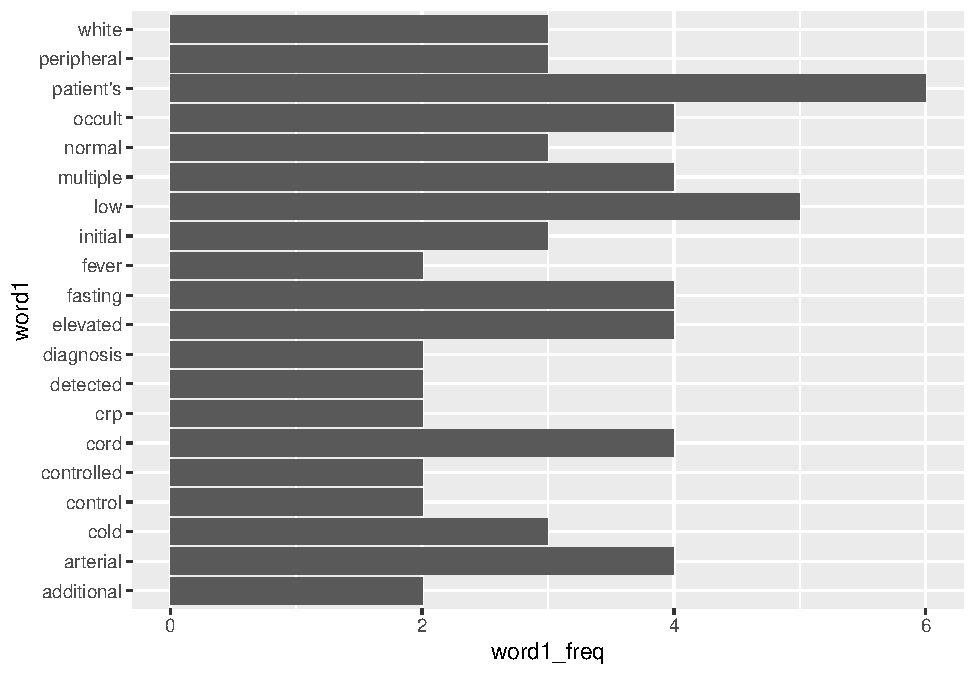
\includegraphics{lab08-text-mining_files/figure-latex/unnamed-chunk-16-1.pdf}

We can also look at which words appear the most frequently AFTER the
word ``blood'':

\begin{Shaded}
\begin{Highlighting}[]
\NormalTok{tokens }\SpecialCharTok{\%\textgreater{}\%}
  \FunctionTok{subset}\NormalTok{(word2 }\SpecialCharTok{==} \StringTok{"blood"}\NormalTok{) }\SpecialCharTok{\%\textgreater{}\%}
  \FunctionTok{group\_by}\NormalTok{(word3) }\SpecialCharTok{\%\textgreater{}\%}
  \FunctionTok{summarise}\NormalTok{(}\AttributeTok{word3\_freq =} \FunctionTok{n}\NormalTok{()) }\SpecialCharTok{\%\textgreater{}\%}
  \FunctionTok{arrange}\NormalTok{(}\FunctionTok{across}\NormalTok{(word3\_freq, desc)) }\SpecialCharTok{\%\textgreater{}\%}
  \FunctionTok{head}\NormalTok{(}\DecValTok{20}\NormalTok{) }\SpecialCharTok{\%\textgreater{}\%}
  \FunctionTok{kable}\NormalTok{() }\SpecialCharTok{\%\textgreater{}\%}
  \FunctionTok{kable\_styling}\NormalTok{()}
\end{Highlighting}
\end{Shaded}

\begin{table}
\centering
\begin{tabular}{l|r}
\hline
word3 & word3\_freq\\
\hline
pressure & 78\\
\hline
loss & 38\\
\hline
cultures & 13\\
\hline
sugar & 13\\
\hline
flow & 11\\
\hline
sugars & 10\\
\hline
pressures & 9\\
\hline
culture & 7\\
\hline
glucose & 6\\
\hline
supply & 5\\
\hline
tests & 5\\
\hline
transfusions & 5\\
\hline
count & 4\\
\hline
return & 4\\
\hline
test & 4\\
\hline
vessels & 4\\
\hline
cell & 3\\
\hline
gas & 3\\
\hline
studies & 3\\
\hline
borne & 2\\
\hline
\end{tabular}
\end{table}

We can again visualize the frequencies:

\begin{Shaded}
\begin{Highlighting}[]
\NormalTok{tokens }\SpecialCharTok{\%\textgreater{}\%}
  \FunctionTok{subset}\NormalTok{(word2 }\SpecialCharTok{==} \StringTok{"blood"}\NormalTok{) }\SpecialCharTok{\%\textgreater{}\%}
  \FunctionTok{group\_by}\NormalTok{(word3) }\SpecialCharTok{\%\textgreater{}\%}
  \FunctionTok{summarise}\NormalTok{(}\AttributeTok{word3\_freq =} \FunctionTok{n}\NormalTok{()) }\SpecialCharTok{\%\textgreater{}\%}
  \FunctionTok{arrange}\NormalTok{(}\FunctionTok{across}\NormalTok{(word3\_freq, desc)) }\SpecialCharTok{\%\textgreater{}\%}
  \FunctionTok{head}\NormalTok{(}\DecValTok{20}\NormalTok{) }\SpecialCharTok{\%\textgreater{}\%}
  \FunctionTok{ggplot}\NormalTok{(}\FunctionTok{aes}\NormalTok{(word3, word3\_freq)) }\SpecialCharTok{+}
  \FunctionTok{geom\_bar}\NormalTok{(}\AttributeTok{stat =} \StringTok{\textquotesingle{}identity\textquotesingle{}}\NormalTok{) }\SpecialCharTok{+}
  \FunctionTok{coord\_flip}\NormalTok{()}
\end{Highlighting}
\end{Shaded}

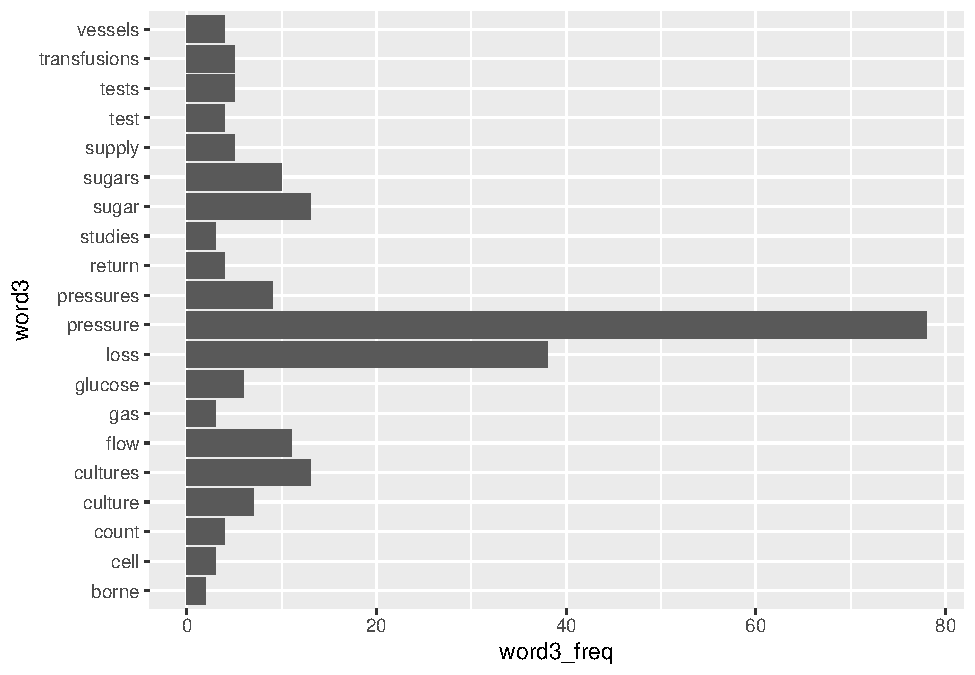
\includegraphics{lab08-text-mining_files/figure-latex/unnamed-chunk-18-1.pdf}

From the visualizations and frequency tables above, we can conclude that
the word that most frequently appears before ``blood'' is ``patient's'',
while the word that most frequently appears after ``blood'' is
``pressure''.

\begin{center}\rule{0.5\linewidth}{0.5pt}\end{center}

\hypertarget{question-6}{%
\section{Question 6}\label{question-6}}

Which words are most used in each of the specialties. you can use
\texttt{group\_by()} and \texttt{top\_n()} from \texttt{dplyr} to have
the calculations be done within each specialty. Remember to remove
stopwords. How about the most 5 used words?

First, we will examine the top words used in each of the specialties:

\begin{Shaded}
\begin{Highlighting}[]
\NormalTok{mt\_samples }\SpecialCharTok{\%\textgreater{}\%}
  \FunctionTok{unnest\_tokens}\NormalTok{(word, transcription) }\SpecialCharTok{\%\textgreater{}\%}
  \FunctionTok{anti\_join}\NormalTok{(stop\_words, }\AttributeTok{by =} \StringTok{"word"}\NormalTok{) }\SpecialCharTok{\%\textgreater{}\%}
  \FunctionTok{subset}\NormalTok{(}\SpecialCharTok{!}\FunctionTok{grepl}\NormalTok{(}\StringTok{"\^{}}\SpecialCharTok{\textbackslash{}\textbackslash{}}\StringTok{d+$"}\NormalTok{, word)) }\SpecialCharTok{\%\textgreater{}\%}
  \FunctionTok{group\_by}\NormalTok{(medical\_specialty) }\SpecialCharTok{\%\textgreater{}\%}
  \FunctionTok{count}\NormalTok{(word, }\AttributeTok{sort =} \ConstantTok{TRUE}\NormalTok{) }\SpecialCharTok{\%\textgreater{}\%}
  \FunctionTok{top\_n}\NormalTok{(}\DecValTok{1}\NormalTok{, n) }\SpecialCharTok{\%\textgreater{}\%}
  \FunctionTok{kable}\NormalTok{() }\SpecialCharTok{\%\textgreater{}\%}
  \FunctionTok{kable\_styling}\NormalTok{()}
\end{Highlighting}
\end{Shaded}

\begin{table}
\centering
\begin{tabular}{l|l|r}
\hline
medical\_specialty & word & n\\
\hline
Surgery & patient & 4855\\
\hline
Consult - History and Phy. & patient & 3046\\
\hline
Orthopedic & patient & 1711\\
\hline
Cardiovascular / Pulmonary & left & 1550\\
\hline
General Medicine & patient & 1356\\
\hline
Gastroenterology & patient & 872\\
\hline
Urology & patient & 776\\
\hline
Radiology & left & 701\\
\hline
Emergency Room Reports & patient & 685\\
\hline
Discharge Summary & patient & 672\\
\hline
Neurology & left & 672\\
\hline
Obstetrics / Gynecology & patient & 628\\
\hline
SOAP / Chart / Progress Notes & patient & 537\\
\hline
Psychiatry / Psychology & patient & 532\\
\hline
Ophthalmology & eye & 456\\
\hline
ENT - Otolaryngology & patient & 415\\
\hline
Neurosurgery & patient & 374\\
\hline
Nephrology & patient & 348\\
\hline
Hematology - Oncology & patient & 316\\
\hline
Pediatrics - Neonatal & patient & 247\\
\hline
Pain Management & patient & 236\\
\hline
Podiatry & foot & 232\\
\hline
Office Notes & normal & 230\\
\hline
Physical Medicine - Rehab & patient & 220\\
\hline
Dentistry & patient & 195\\
\hline
Chiropractic & pain & 187\\
\hline
IME-QME-Work Comp etc. & pain & 152\\
\hline
Sleep Medicine & sleep & 143\\
\hline
Endocrinology & thyroid & 129\\
\hline
Cosmetic / Plastic Surgery & patient & 116\\
\hline
Speech - Language & patient & 105\\
\hline
Dermatology & patient & 101\\
\hline
Dermatology & skin & 101\\
\hline
Autopsy & left & 83\\
\hline
Letters & pain & 80\\
\hline
Bariatrics & patient & 62\\
\hline
Rheumatology & history & 50\\
\hline
Diets and Nutritions & patient & 43\\
\hline
Hospice - Palliative Care & patient & 43\\
\hline
Allergy / Immunology & history & 38\\
\hline
Lab Medicine - Pathology & cm & 35\\
\hline
Lab Medicine - Pathology & tumor & 35\\
\hline
\end{tabular}
\end{table}

Above, we have a table describing which word is used most frequently in
each specialty and how frequently the specialty occurs. Next, we can
look at the top 5 most frequently used words for each specialty:

\begin{Shaded}
\begin{Highlighting}[]
\NormalTok{mt\_samples }\SpecialCharTok{\%\textgreater{}\%}
  \FunctionTok{unnest\_tokens}\NormalTok{(word, transcription) }\SpecialCharTok{\%\textgreater{}\%}
  \FunctionTok{anti\_join}\NormalTok{(stop\_words, }\AttributeTok{by =} \StringTok{"word"}\NormalTok{) }\SpecialCharTok{\%\textgreater{}\%}
  \FunctionTok{subset}\NormalTok{(}\SpecialCharTok{!}\FunctionTok{grepl}\NormalTok{(}\StringTok{"\^{}}\SpecialCharTok{\textbackslash{}\textbackslash{}}\StringTok{d+$"}\NormalTok{, word)) }\SpecialCharTok{\%\textgreater{}\%}
  \FunctionTok{group\_by}\NormalTok{(medical\_specialty) }\SpecialCharTok{\%\textgreater{}\%}
  \FunctionTok{count}\NormalTok{(word) }\SpecialCharTok{\%\textgreater{}\%}
  \FunctionTok{top\_n}\NormalTok{(}\DecValTok{5}\NormalTok{, n) }\SpecialCharTok{\%\textgreater{}\%}
  \FunctionTok{kable}\NormalTok{() }\SpecialCharTok{\%\textgreater{}\%}
  \FunctionTok{kable\_styling}\NormalTok{()}
\end{Highlighting}
\end{Shaded}

\begin{table}
\centering
\begin{tabular}{l|l|r}
\hline
medical\_specialty & word & n\\
\hline
Allergy / Immunology & allergies & 21\\
\hline
Allergy / Immunology & history & 38\\
\hline
Allergy / Immunology & nasal & 13\\
\hline
Allergy / Immunology & noted & 23\\
\hline
Allergy / Immunology & past & 13\\
\hline
Allergy / Immunology & patient & 22\\
\hline
Autopsy & anterior & 47\\
\hline
Autopsy & body & 40\\
\hline
Autopsy & inch & 59\\
\hline
Autopsy & left & 83\\
\hline
Autopsy & neck & 55\\
\hline
Bariatrics & gastric & 30\\
\hline
Bariatrics & history & 50\\
\hline
Bariatrics & patient & 62\\
\hline
Bariatrics & surgery & 34\\
\hline
Bariatrics & weight & 36\\
\hline
Cardiovascular / Pulmonary & artery & 1085\\
\hline
Cardiovascular / Pulmonary & coronary & 681\\
\hline
Cardiovascular / Pulmonary & history & 654\\
\hline
Cardiovascular / Pulmonary & left & 1550\\
\hline
Cardiovascular / Pulmonary & patient & 1516\\
\hline
Chiropractic & dr & 66\\
\hline
Chiropractic & history & 56\\
\hline
Chiropractic & left & 54\\
\hline
Chiropractic & pain & 187\\
\hline
Chiropractic & patient & 85\\
\hline
Consult - History and Phy. & history & 2820\\
\hline
Consult - History and Phy. & mg & 908\\
\hline
Consult - History and Phy. & normal & 1368\\
\hline
Consult - History and Phy. & pain & 1153\\
\hline
Consult - History and Phy. & patient & 3046\\
\hline
Cosmetic / Plastic Surgery & breast & 95\\
\hline
Cosmetic / Plastic Surgery & incision & 67\\
\hline
Cosmetic / Plastic Surgery & patient & 116\\
\hline
Cosmetic / Plastic Surgery & procedure & 98\\
\hline
Cosmetic / Plastic Surgery & skin & 88\\
\hline
Dentistry & left & 94\\
\hline
Dentistry & patient & 195\\
\hline
Dentistry & procedure & 82\\
\hline
Dentistry & teeth & 104\\
\hline
Dentistry & tooth & 108\\
\hline
Dermatology & cm & 77\\
\hline
Dermatology & left & 58\\
\hline
Dermatology & patient & 101\\
\hline
Dermatology & procedure & 44\\
\hline
Dermatology & skin & 101\\
\hline
Diets and Nutritions & carbohydrate & 37\\
\hline
Diets and Nutritions & day & 28\\
\hline
Diets and Nutritions & food & 27\\
\hline
Diets and Nutritions & patient & 43\\
\hline
Diets and Nutritions & plan & 27\\
\hline
Diets and Nutritions & weight & 40\\
\hline
Discharge Summary & discharge & 358\\
\hline
Discharge Summary & history & 208\\
\hline
Discharge Summary & hospital & 183\\
\hline
Discharge Summary & mg & 301\\
\hline
Discharge Summary & patient & 672\\
\hline
Emergency Room Reports & denies & 149\\
\hline
Emergency Room Reports & history & 356\\
\hline
Emergency Room Reports & normal & 255\\
\hline
Emergency Room Reports & pain & 273\\
\hline
Emergency Room Reports & patient & 685\\
\hline
Endocrinology & dissection & 45\\
\hline
Endocrinology & gland & 45\\
\hline
Endocrinology & history & 57\\
\hline
Endocrinology & left & 63\\
\hline
Endocrinology & nerve & 45\\
\hline
Endocrinology & patient & 121\\
\hline
Endocrinology & thyroid & 129\\
\hline
ENT - Otolaryngology & ear & 182\\
\hline
ENT - Otolaryngology & left & 219\\
\hline
ENT - Otolaryngology & nasal & 281\\
\hline
ENT - Otolaryngology & patient & 415\\
\hline
ENT - Otolaryngology & procedure & 181\\
\hline
Gastroenterology & colon & 240\\
\hline
Gastroenterology & history & 341\\
\hline
Gastroenterology & normal & 328\\
\hline
Gastroenterology & patient & 872\\
\hline
Gastroenterology & procedure & 470\\
\hline
General Medicine & history & 1027\\
\hline
General Medicine & mg & 503\\
\hline
General Medicine & normal & 717\\
\hline
General Medicine & pain & 567\\
\hline
General Medicine & patient & 1356\\
\hline
Hematology - Oncology & history & 290\\
\hline
Hematology - Oncology & left & 187\\
\hline
Hematology - Oncology & mass & 97\\
\hline
Hematology - Oncology & mg & 107\\
\hline
Hematology - Oncology & patient & 316\\
\hline
Hospice - Palliative Care & daughter & 22\\
\hline
Hospice - Palliative Care & family & 19\\
\hline
Hospice - Palliative Care & history & 27\\
\hline
Hospice - Palliative Care & mg & 28\\
\hline
Hospice - Palliative Care & pain & 19\\
\hline
Hospice - Palliative Care & patient & 43\\
\hline
IME-QME-Work Comp etc. & dr & 82\\
\hline
IME-QME-Work Comp etc. & injury & 81\\
\hline
IME-QME-Work Comp etc. & left & 70\\
\hline
IME-QME-Work Comp etc. & pain & 152\\
\hline
IME-QME-Work Comp etc. & patient & 106\\
\hline
Lab Medicine - Pathology & cm & 35\\
\hline
Lab Medicine - Pathology & lobe & 29\\
\hline
Lab Medicine - Pathology & lymph & 30\\
\hline
Lab Medicine - Pathology & tumor & 35\\
\hline
Lab Medicine - Pathology & upper & 20\\
\hline
Letters & abc & 71\\
\hline
Letters & dr & 46\\
\hline
Letters & normal & 53\\
\hline
Letters & pain & 80\\
\hline
Letters & patient & 65\\
\hline
Nephrology & history & 160\\
\hline
Nephrology & kidney & 144\\
\hline
Nephrology & left & 132\\
\hline
Nephrology & patient & 348\\
\hline
Nephrology & renal & 257\\
\hline
Neurology & history & 429\\
\hline
Neurology & left & 672\\
\hline
Neurology & normal & 485\\
\hline
Neurology & patient & 648\\
\hline
Neurology & time & 278\\
\hline
Neurosurgery & c5 & 289\\
\hline
Neurosurgery & c6 & 266\\
\hline
Neurosurgery & left & 222\\
\hline
Neurosurgery & patient & 374\\
\hline
Neurosurgery & procedure & 247\\
\hline
Obstetrics / Gynecology & incision & 293\\
\hline
Obstetrics / Gynecology & normal & 276\\
\hline
Obstetrics / Gynecology & patient & 628\\
\hline
Obstetrics / Gynecology & procedure & 301\\
\hline
Obstetrics / Gynecology & uterus & 317\\
\hline
Office Notes & history & 76\\
\hline
Office Notes & negative & 193\\
\hline
Office Notes & normal & 230\\
\hline
Office Notes & noted & 60\\
\hline
Office Notes & patient & 94\\
\hline
Ophthalmology & anterior & 150\\
\hline
Ophthalmology & chamber & 149\\
\hline
Ophthalmology & eye & 456\\
\hline
Ophthalmology & patient & 258\\
\hline
Ophthalmology & procedure & 176\\
\hline
Orthopedic & lateral & 472\\
\hline
Orthopedic & left & 998\\
\hline
Orthopedic & pain & 763\\
\hline
Orthopedic & patient & 1711\\
\hline
Orthopedic & procedure & 669\\
\hline
Pain Management & injected & 76\\
\hline
Pain Management & needle & 156\\
\hline
Pain Management & pain & 76\\
\hline
Pain Management & patient & 236\\
\hline
Pain Management & procedure & 197\\
\hline
Pediatrics - Neonatal & child & 82\\
\hline
Pediatrics - Neonatal & history & 235\\
\hline
Pediatrics - Neonatal & mom & 82\\
\hline
Pediatrics - Neonatal & normal & 155\\
\hline
Pediatrics - Neonatal & patient & 247\\
\hline
Physical Medicine - Rehab & history & 54\\
\hline
Physical Medicine - Rehab & left & 104\\
\hline
Physical Medicine - Rehab & motor & 62\\
\hline
Physical Medicine - Rehab & pain & 95\\
\hline
Physical Medicine - Rehab & patient & 220\\
\hline
Podiatry & foot & 232\\
\hline
Podiatry & incision & 96\\
\hline
Podiatry & left & 137\\
\hline
Podiatry & patient & 231\\
\hline
Podiatry & tendon & 98\\
\hline
Psychiatry / Psychology & history & 344\\
\hline
Psychiatry / Psychology & mg & 183\\
\hline
Psychiatry / Psychology & mother & 164\\
\hline
Psychiatry / Psychology & patient & 532\\
\hline
Psychiatry / Psychology & reported & 141\\
\hline
Radiology & exam & 302\\
\hline
Radiology & left & 701\\
\hline
Radiology & mild & 242\\
\hline
Radiology & normal & 644\\
\hline
Radiology & patient & 304\\
\hline
Rheumatology & day & 22\\
\hline
Rheumatology & examination & 22\\
\hline
Rheumatology & history & 50\\
\hline
Rheumatology & joints & 22\\
\hline
Rheumatology & mg & 26\\
\hline
Rheumatology & pain & 23\\
\hline
Rheumatology & patient & 34\\
\hline
Sleep Medicine & activity & 31\\
\hline
Sleep Medicine & apnea & 35\\
\hline
Sleep Medicine & patient & 69\\
\hline
Sleep Medicine & sleep & 143\\
\hline
Sleep Medicine & stage & 29\\
\hline
SOAP / Chart / Progress Notes & blood & 194\\
\hline
SOAP / Chart / Progress Notes & history & 254\\
\hline
SOAP / Chart / Progress Notes & mg & 302\\
\hline
SOAP / Chart / Progress Notes & pain & 239\\
\hline
SOAP / Chart / Progress Notes & patient & 537\\
\hline
Speech - Language & evaluation & 17\\
\hline
Speech - Language & goals & 17\\
\hline
Speech - Language & patient & 105\\
\hline
Speech - Language & patient's & 28\\
\hline
Speech - Language & speech & 35\\
\hline
Speech - Language & term & 17\\
\hline
Speech - Language & therapy & 41\\
\hline
Speech - Language & time & 17\\
\hline
Surgery & anesthesia & 1687\\
\hline
Surgery & incision & 1641\\
\hline
Surgery & left & 3263\\
\hline
Surgery & patient & 4855\\
\hline
Surgery & procedure & 3243\\
\hline
Urology & bladder & 357\\
\hline
Urology & history & 196\\
\hline
Urology & left & 288\\
\hline
Urology & patient & 776\\
\hline
Urology & procedure & 306\\
\hline
\end{tabular}
\end{table}

\hypertarget{question-7---extra}{%
\section{Question 7 - extra}\label{question-7---extra}}

Find your own insight in the data:

Ideas:

\begin{itemize}
\tightlist
\item
  Interesting ngrams
\item
  See if certain words are used more in some specialties then others
\end{itemize}

\hypertarget{deliverables}{%
\section{Deliverables}\label{deliverables}}

\begin{enumerate}
\def\labelenumi{\arabic{enumi}.}
\tightlist
\item
  Questions 1-7 answered, pdf or html output uploaded to quercus
\end{enumerate}

\end{document}
